\chapter{Исследовательская часть}
В данной части будет проведено исследование влияния индекса на время выполнения запросов к базе данных.

\section{Описание исследования}
Индекс -- это объект базы данных, который обеспечивает дополнительные способы поиска и извлечения данных. Индекс может создаваться на одном или нескольких столбцах. 

Для исследовании будет использован тип индекса B--дерево. B--дерево является самой распространенной индексной структурой и состоит из иерархически организованных узлов, связанных с блоками, хранящимися на диске~\cite{dombrovskaya}.


Замеры времени выполнения запросов будут проводиться с использованием функции $time.perf\_counter$~\cite{timeperf} языка $Python$~\cite{Python}.


\section{Технические характеристики устройства}
Технические характеристики устройства, на котором проводилось исследование:
\begin{itemize}
	\item операционная система Windows 11 64-разрядная операционная система;
	\item оперативная память 16 ГБ;
	\item процессор AMD Ryzen 5 5600U with Radeon Graphics 2.30 ГГц.
\end{itemize}


\section{Результаты исследования}
\subsection{Поиск по полю с фильтрацией}
Для создания индекса использовалась команда:
\begin{lstlisting}[language=SQL]
	CREATE INDEX index_users_birthdate ON users using btree(birthdate)
\end{lstlisting}


В таблице~\ref{birthdate_table} представлены результаты замеров времени выполнения запроса в миллисекундах.


\newpage
\begin{table}[ht]
	\begin{center}
		\begin{threeparttable}
			\caption{\label{birthdate_table} Время выполнения запроса в миллисекундах}
			\begin{tabular}{|p{7cm}|p{4cm}|p{4cm}|c|}
				\hline
				\textbf{Количество записей в таблице} & \textbf{Без индекса} & {\textbf{С индексом}} \\ \hline
				1000 & 0.178 & 0.139 \\ \hline
				5000 & 0.398 & 0.168 \\ \hline
				10000 & 0.705 & 0.172 \\ \hline
				25000 & 1.601 & 0.169 \\ \hline
				50000 & 3.213 & 0.184 \\ \hline
				100000 & 7.403 & 0.173 \\ \hline
				250000 & 17.551 & 0.176 \\ \hline
			\end{tabular}
		\end{threeparttable}
	\end{center}
\end{table}

На рисунке ~\ref{birth_graph} приведены результаты замеров времени выполнения запроса в виде графика.

\begin{figure}[H]
	\centering
	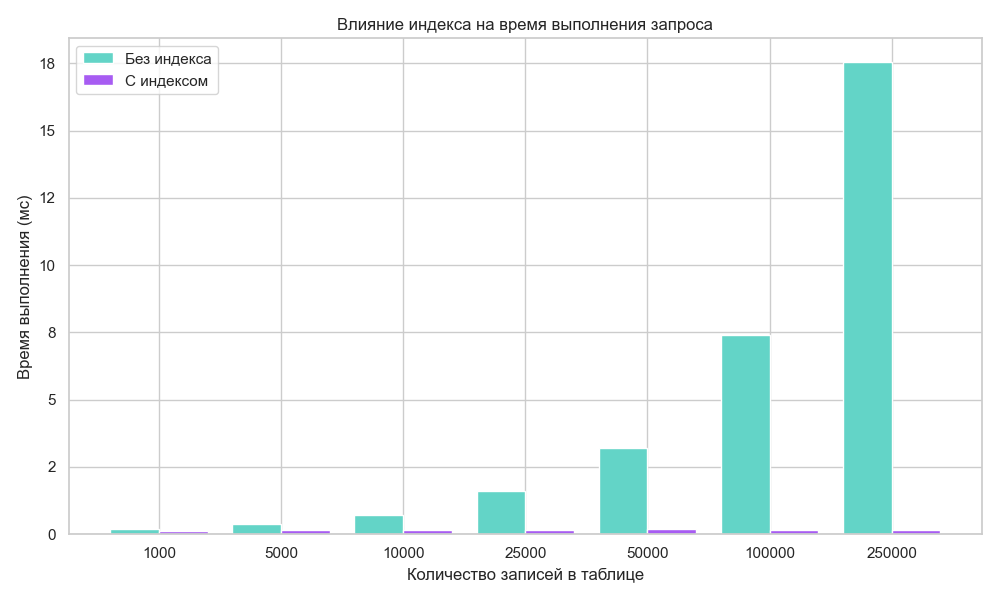
\includegraphics[width=1\linewidth]{img/graph_select_birthdate.png}
	\caption{Исследование влияния индекса на время выполнения запроса}
	\label{birth_graph}
\end{figure}


По результатам исследования сделан вывод о том, что использование индекса позволяет уменьшить время выполнения запросов к базе данных.
Согласно полученным замерам, время выполнения запроса максимально сократилось примерно в 100 раз.
  Такой результат связан с тем, что при отсутствии индекса поиск нужных данных в таблице выполняется простым сканированием всех ее строк.

\subsection{Поиск по первичному ключу}
Для создания индекса использовалась команда:
\begin{lstlisting}[language=SQL]
	CREATE INDEX index_users_id ON users using btree(id_user)
\end{lstlisting}

В таблице~\ref{id_table} представлены результаты замеров времени выполнения в миллисекундах.


\begin{table}[ht]
	\begin{center}
		\begin{threeparttable}
			\caption{\label{id_table} Время выполнения запроса в миллисекундах}
			\begin{tabular}{|p{7cm}|p{4cm}|p{4cm}|c|}
				\hline
				\textbf{Количество записей в таблице} & \textbf{Без индекса} & {С индексом} \\ \hline
				1000 & 0.105 & 0.149 \\ \hline
				5000 & 0.100 & 0.151 \\ \hline
				10000 & 0.119 & 0.170 \\ \hline
				25000 & 0.107 & 0.160 \\ \hline
				50000 & 0.120 & 0.171 \\ \hline
				100000 & 0.118 & 0.161 \\ \hline
				250000 & 0.135 & 0.154 \\ \hline
				
			\end{tabular}
		\end{threeparttable}
	\end{center}
\end{table}


На рисунке ~\ref{id_graph} приведены результаты замеров времени выполнения запроса в виде графика.

\begin{figure}[H]
	\centering
	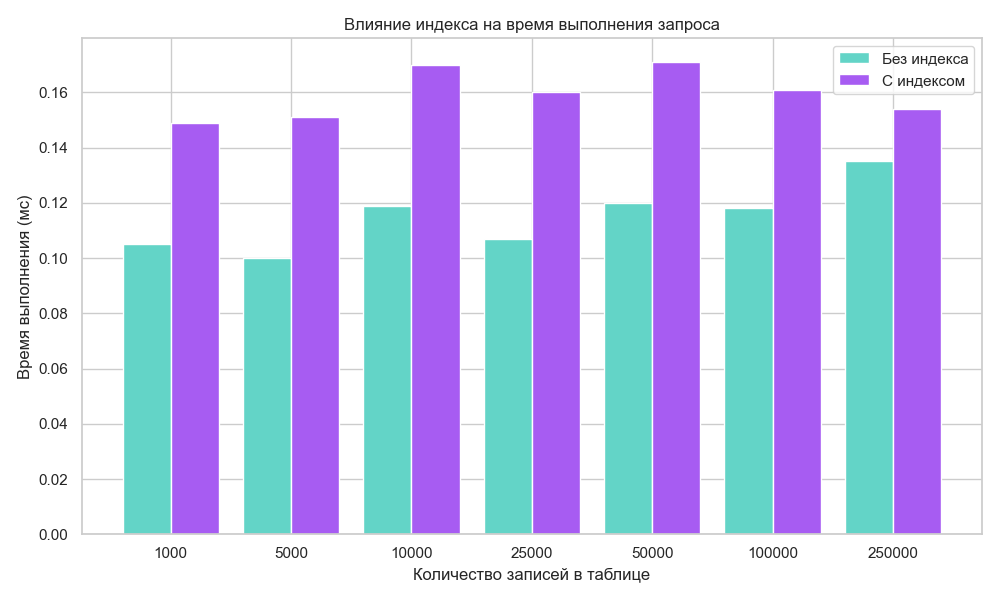
\includegraphics[width=1\linewidth]{img/graph_id.png}
	\caption{Исследование влияния индекса на время выполнения запроса}
	\label{id_graph}
\end{figure}

По результатам исследования сделан вывод о том, что использование индекса не сократило время выполнения запроса. Полученный результат связан с тем, что при создании таблиц для столбца первичного ключа автоматически создается индекс и создание дополнительного индекса на данное поле избыточно. 




\section*{Вывод}
В данной части было проведено исследование влияния индекса на время выполнения запросов к базе данных. По результатам проведенных замеров сделан вывод о том, что наличие индекса позволяет уменьшить время поиска нужных строк в таблице. В то же время создание индексов для первичных ключей не приводит к повышению эффективности, поскольку индексы для этих полей создаются автоматически.